\subsection{Prototypical Implementation}
\label{subsec:prototype}


%
%The first step of the approach is the preprocess of the VCS log received as input. The main goal of this phase is generate a set of events and store them into a database. Second, we obtain different views on the stored events. In particular, we are interested in observing
%\begin{inparaenum}[\itshape i)]
%	\item all the commits that affected the files over time;
%	\item the amount of change brought by the commits to the files; and
%	\item the users who issued such commits.
%\end{inparaenum}
%The third phase is responsible for considering the different perspectives defined by the project manager and through the generated views extract the necessary knowledge. The last phase is responsible for providing the visualization combining the different perspectives considered. The following sections detail each of the phases.

We implemented our technique as a prototype\footnote{\url{https://github.com/s41m1r/MiningVCS.git}}. The input of our program is a \gls{vcs} log and the output is a set of analysis data with information about the evolution of the artifacts and their dependencies. 
%%Next we show the implementation details of \Cref{algorithm:all}.
%
%
%
%%\subsubsection{Preprocess VCS Logs.}
%As a first step (cf.~\Cref{algorithm:all}) we need to preprocess the input in order to extract events. Events in \gls{vcs} have multiple dimensions and relations among one another. Therefore, the natural way of capturing them is through a relational data model. This model serves at structuring the raw data and persisting the results after first step of \Cref{algorithm:all}. \Cref{fig:data-model} outlines the main entities in a \gls{vcs} and the relationships of our interest. The result the first step of \Cref{algorithm:all} is the correct population of the a database with the set of the extracted events, stored according to the relational schema. 
%
%\begin{figure}[]
%	\centering
%	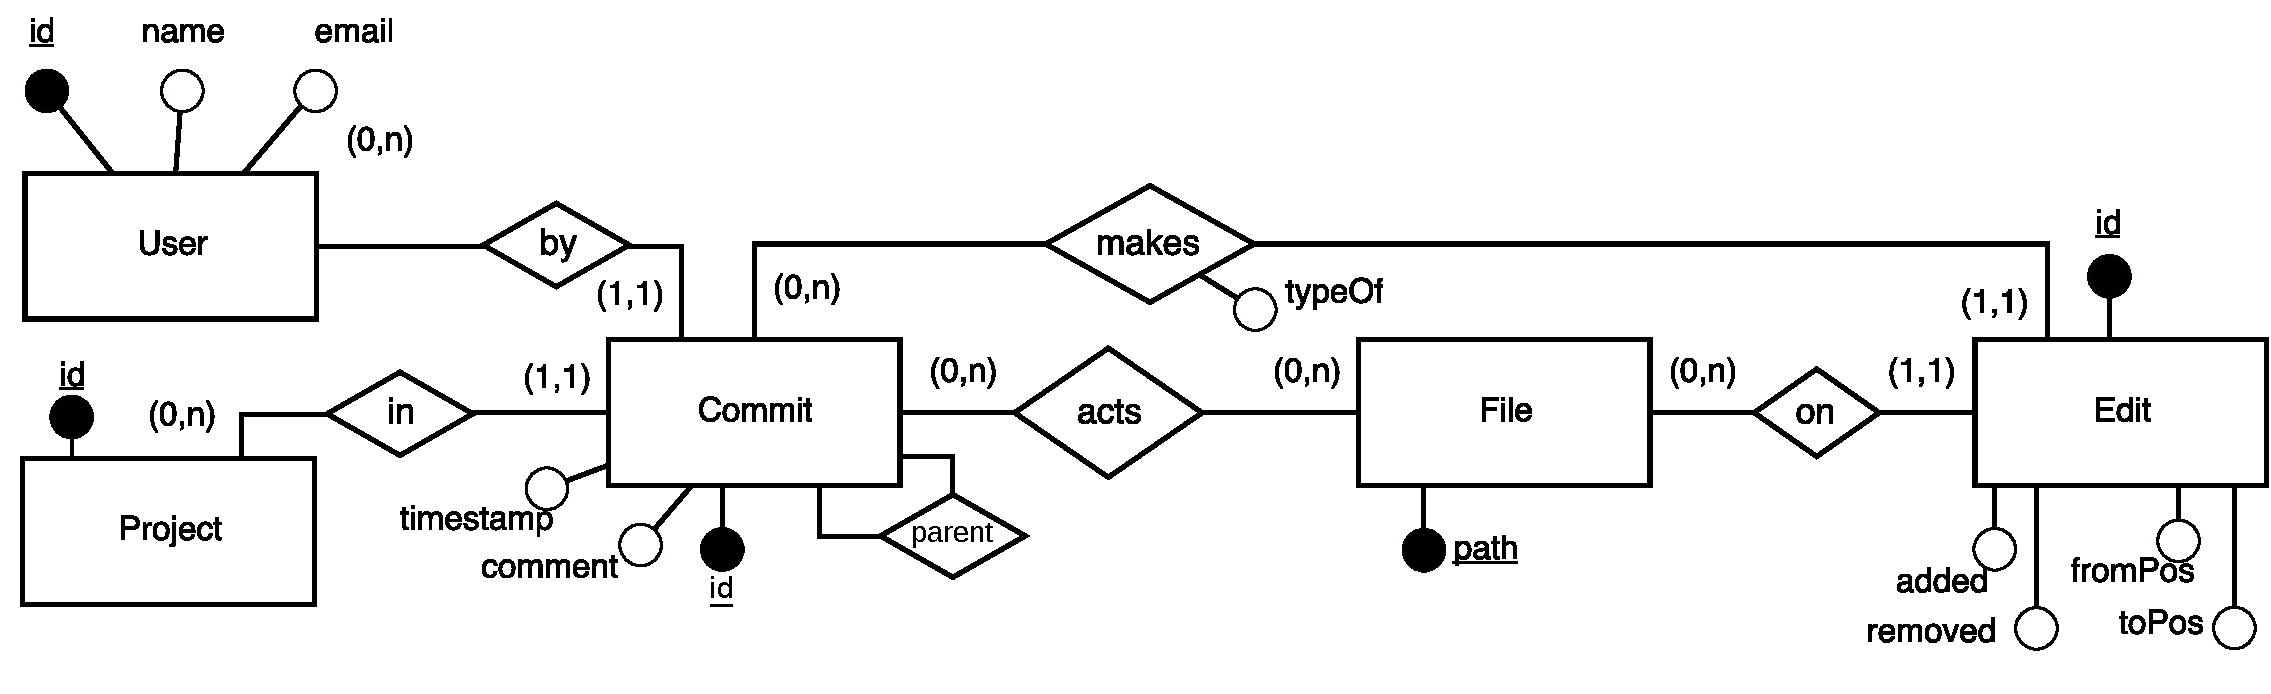
\includegraphics[width=0.9\linewidth]{figures/CommitLogER}
%	\caption{Relational schema of a software project}
%	\label{fig:data-model}
%\end{figure}
%
%%\subsubsection{Obtain View on Project.}
%
%The step~\ref{algorithm:all} makes queries over the event set in order to retrieve aggregated views from them. This is simply done by defining queries on the database and export collect their results (e.g., in a CSV file). Step~\ref{step:contaiments} consists in recreating the file structure. This is implemented by reverse engineering the directory structure from the \texttt{path} attribute of the entity \texttt{File} that is present in the output of the query. Next, we actuate step~\ref{step:evolution} by implementing \Cref{algorithm:compute-evolution} that computes the artifact evolutions. This algorithm takes as input the set of views calculated previously and outputs \begin{inparaenum}[\itshape i)]
%	\item and a set of \emph{file stories} that report the amount of change, time and comments of the file history, and
%	\item a set process that describe the evolution of every artifact obtained by story mining~\cite{Goncalves2011} the file stories.
%\end{inparaenum} Finally, for step~\ref{step:dependencies} we implement \Cref{algorithm:compute-dependencies}. This algorithm takes as input the aggregated views obtained previously and two parameters: a comparison function and a threshold. We use the Pearson correlation $\rho$ and let the domain expert set the threshold $\delta$ to filter the strength of the dependencies. An important step before 


%One example of query that outputs a view of the daily changes of the artifact \texttt{model.java} is shown in \Cref{lst:query}. 

%\begin{center}
%\begin{lstlisting}[
%language=SQL,
%showspaces=false,
%float=ht,
%xleftmargin=4em,
%aboveskip=6pt,
%belowskip=0cm,
%belowcaptionskip=0cm,
%basicstyle=\ttfamily\scriptsize,
%showstringspaces=false,
%commentstyle=\color{gray},
%mathescape=true,
%caption={SQL query to obtain the artifact history for a given artifact, aggregated on a day level},captionpos=b, label={lst:query}
%]
%SELECT CONCAT(Commit.comment,$\S$) as Comments, 
%	DATE(Commit.timeStamp) as Date, 
%	sum(linesAdded+linesRemoved) as Change, 
%	CONCAT(User.name, '$\S$') as Users
%FROM File, Edit, acts,Commit,User 
%WHERE File.path = 'model.txt' 
%	AND Edit.commit_id = Commit.id 
%	AND Edit.file_path = File.path
%	AND User.id = Commit.user_id
%	AND acts.file_path = File.path 
%	AND acts.commit_id = Commit.id
%GROUP BY Date
%ORDER By Date ASC
%\end{lstlisting}
%\end{center}
%
%\Cref{table:analysis-data} depicts a view obtained with the query in \Cref{lst:query} on the project shown in \Cref{subsec:scenario}. The data is aggregated by day. String values are concatenated together with the symbol '$\S$'.
%
%% Please add the following required packages to your document preamble:
% \usepackage{booktabs}
% \usepackage{graphicx}
\begin{table}[h]
\centering
\caption{View generated by the query in \Cref{lst:query}. Comments and users that affected the artifact at the same day are aggregated by concatenation.}
\label{table:analysis-data}
%\resizebox{\linewidth}{!}{%
\setlength{\tabcolsep}{4pt}
\begin{tabular}{@{}llllllll@{\hspace*{3pt}}}
%\toprule
Comments                                                                                                                                                                            & Date      & \rot{\#LinesAdded} & \rot{\#LinesRemoved} & \rot{TotalChange} & \rot{TotalDiff} & \rot{LinesNow} & \rot{Users}                     \\ \midrule
\rowcolor{lightgray} \begin{tabular}[c]{@{}l@{}}Modify method A to\\  meet the new requirement \\ for methods speed . \\Fix bug on  method A . \\ Create model.java . \\ Add solver methods\end{tabular} & 2017-01-31 & 36              & 1                 & 37                  & 35                & 113               & \begin{tabular}[c]{@{}l@{}}Anna  \\ John  \\ Beth  \end{tabular} \\
Implement method B                                                                                                                                                                      & 2017-02-02 & 21              & 0                 & 21                  & 21                & 56                & Anna                      \\ \rowcolor{lightgray}
Update model.java                                                                                                                                                                       & 2017-02-08 & 25              & 0                 & 25                  & 25                & 81                & Anna                      \\ \bottomrule
\end{tabular}%
%}

\end{table}

%\subsubsection{Analyze project data.}

%The input of this phase is a collection resulting from querying all the artifact histories from the data store. At this point the data is ready to be analyzed. 
%In this step analyses on the view extracted are performed. There are a number of different analyses that can be applied directly to the \emph{aggregate events}, e.g. checking whether project participants have been working on the assigned tasks ("Are they working in the artifacts they should/?") or there has rather been disorganization in regards. In this work, we focus on analyzes related to the artifacts, i.e. how they evolve over time, how they are organized and how are the dependencies among them. Therefore, in this section we focus on extracting the \emph{containments}, \emph{dependencies} and \emph{artifact evolution} elements.
%
%Analyzing the \emph{Parent} relation, the set $C$ of containments for our scenario of use is: $C = \{f_1, f_3, f_4, f_6, f_9, f_{10}\}$. 
%
%\begin{table}[t]
%%	\centering
%	\caption{Time series similarity among the six artifacts}
%	\label{table:time-series-all}
%	\begin{subtable}{.45\linewidth}
%		% Please add the following required packages to your document preamble:
% \usepackage{booktabs}
%\begin{table}[]
\centering
%\caption{Amount of change time series for each of the 6 artifacts in our scenario of use.}
%\caption{}
\label{table:time-series}
\begin{tabular}{@{}crrrrrr@{}}
	\toprule
	Day        & ${f_2}$ & ${f_5}$ & ${f_7}$ & ${f_8}$ & ${f_{11}}$ & ${f_{12}}$ \\ \midrule
	2017-01-31 & 5       & 16      & 37      & 24      & 0          & 2          \\
	2017-02-01 & 0       & 0       & 0       & 0       & 0          & 0          \\
	2017-02-02 & 0       & 2       & 5       & 5       & 0          & 0          \\
	2017-02-03 & 0       & 0       & 4       & 4       & 0          & 0          \\
	2017-02-04 & 0       & 0       & 0       & 0       & 0          & 0          \\
	2017-02-05 & 0       & 0       & 0       & 0       & 0          & 0          \\
	2017-02-06 & 0       & 1       & 25      & 20      & 0          & 0          \\
	2017-02-07 & 0       & 1       & 10      & 9       & 0          & 0          \\
	2017-02-08 & 0       & 0       & 0       & 0       & 0          & 0          \\
	2017-02-09 & 0       & 0       & 25      & 15      & 0          & 0          \\
	2017-02-10 & 1       & 0       & 0       & 0       & 6          & 0          \\ \bottomrule
\end{tabular}%
%\end{table}
%	\end{subtable}
%	\begin{subtable}{.45\linewidth}
%		% Please add the following required packages to your document preamble:
% \usepackage{booktabs}
% \usepackage{graphicx}
%\begin{table}[]
\centering
%\caption{The correlations matrix for the 6 artifacts.}
%\caption{}
\label{table:correlations}
%\resizebox{\textwidth}{!}{%
\begin{tabular}{@{}crrrrrr@{}}
\toprule
$\sigma(f_1,f_2)$ & ${f_2}$ & ${f_5}$ & ${f_7}$ & ${f_8}$ & ${f_{11}}$ & ${f_{12}}$ \\ \midrule 
${f_2}$      & 1.00    &         &         &         &            &            \\
${f_5}$      & 0.96    & 1.00    &         &         &            &            \\
${f_7}$      & 0.64    & 0.71    & 1.00    &         &            &            \\
${f_8}$      & 0.58    & 0.67    & 0.99    & 1.00    &            &            \\
${f_{11}}$   & 0.10    & -0.13   & -0.24   & -0.26   & 1.00       &            \\
${f_{12}}$   & 0.98    & 0.99    & 0.69    & 0.64    & -0.10      & 1.00       \\ \bottomrule
\end{tabular}%
%}

%\end{table}
%	\end{subtable}
%\end{table}
%
%To compute the dependencies, we analyzed the time series depicted in \Cref{table:time-series} computing the correlations pairwise. Considering that the project manger specified a threshold of 0.7, we found the dependencies: \{(${f_7}$,${f_5}$), (${f_7}$,${f_8}$), (${f_2}$,${f_5}$), (${f_2}$,${f_{12}}$), (${f_5}$,${f_{12}}$)\}.
%
%The last step in this phase is the computation of the artifacts evolution. For all 6 artifacts a story containing the comments observed in the aggregate events for that artifact was generated. In the end, six stories were created and for each of them our approach for artifact mining was applied. 
